\section{am::lambda::binder0$<$ R $>$ Struct Template Reference}
\label{structam_1_1lambda_1_1binder0}\index{am::lambda::binder0@{am::lambda::binder0}}
{\tt \#include $<$lambda.hpp$>$}

Inherits {\bf am::lambda::detail::lambda\_\-op\_\-tag}.

Inheritance diagram for am::lambda::binder0$<$ R $>$:\begin{figure}[H]
\begin{center}
\leavevmode
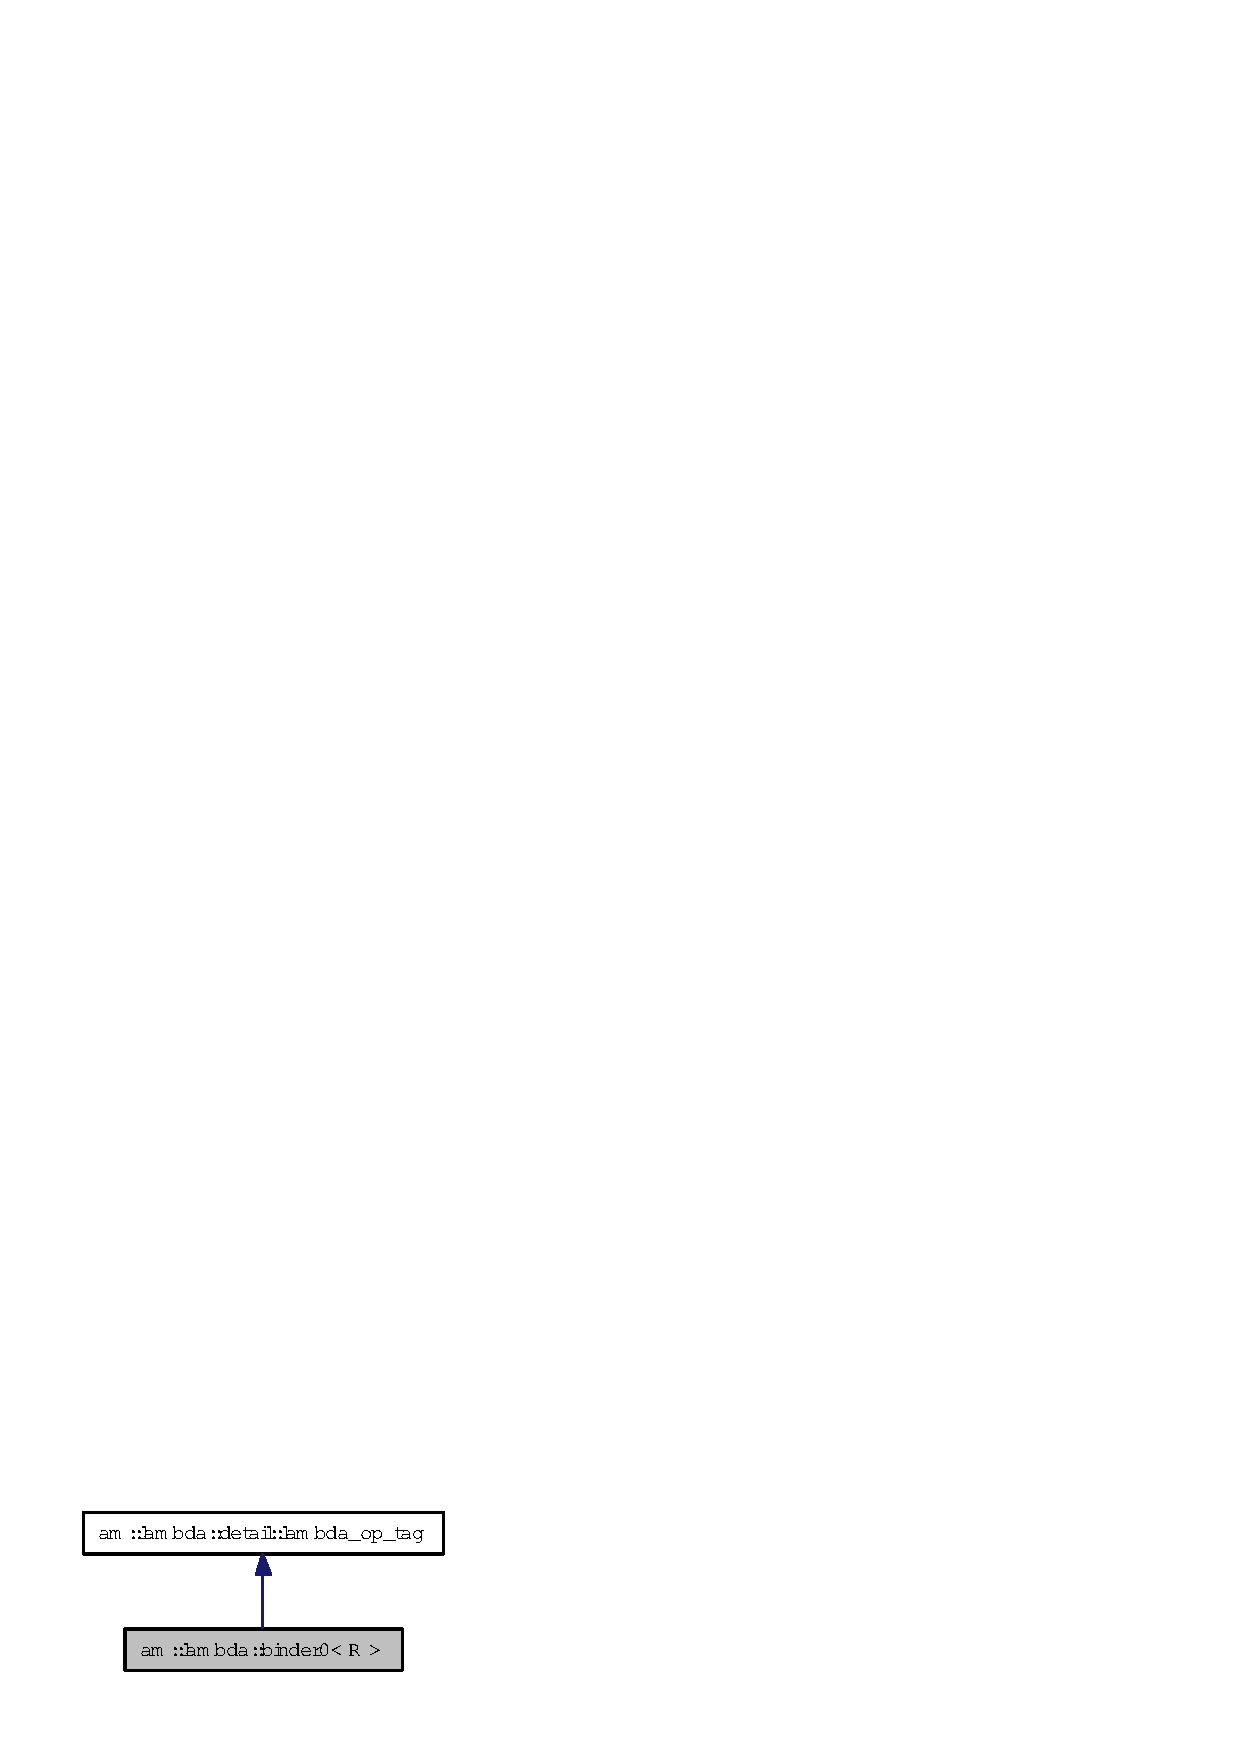
\includegraphics[width=108pt]{structam_1_1lambda_1_1binder0__inherit__graph}
\end{center}
\end{figure}
Collaboration diagram for am::lambda::binder0$<$ R $>$:\begin{figure}[H]
\begin{center}
\leavevmode
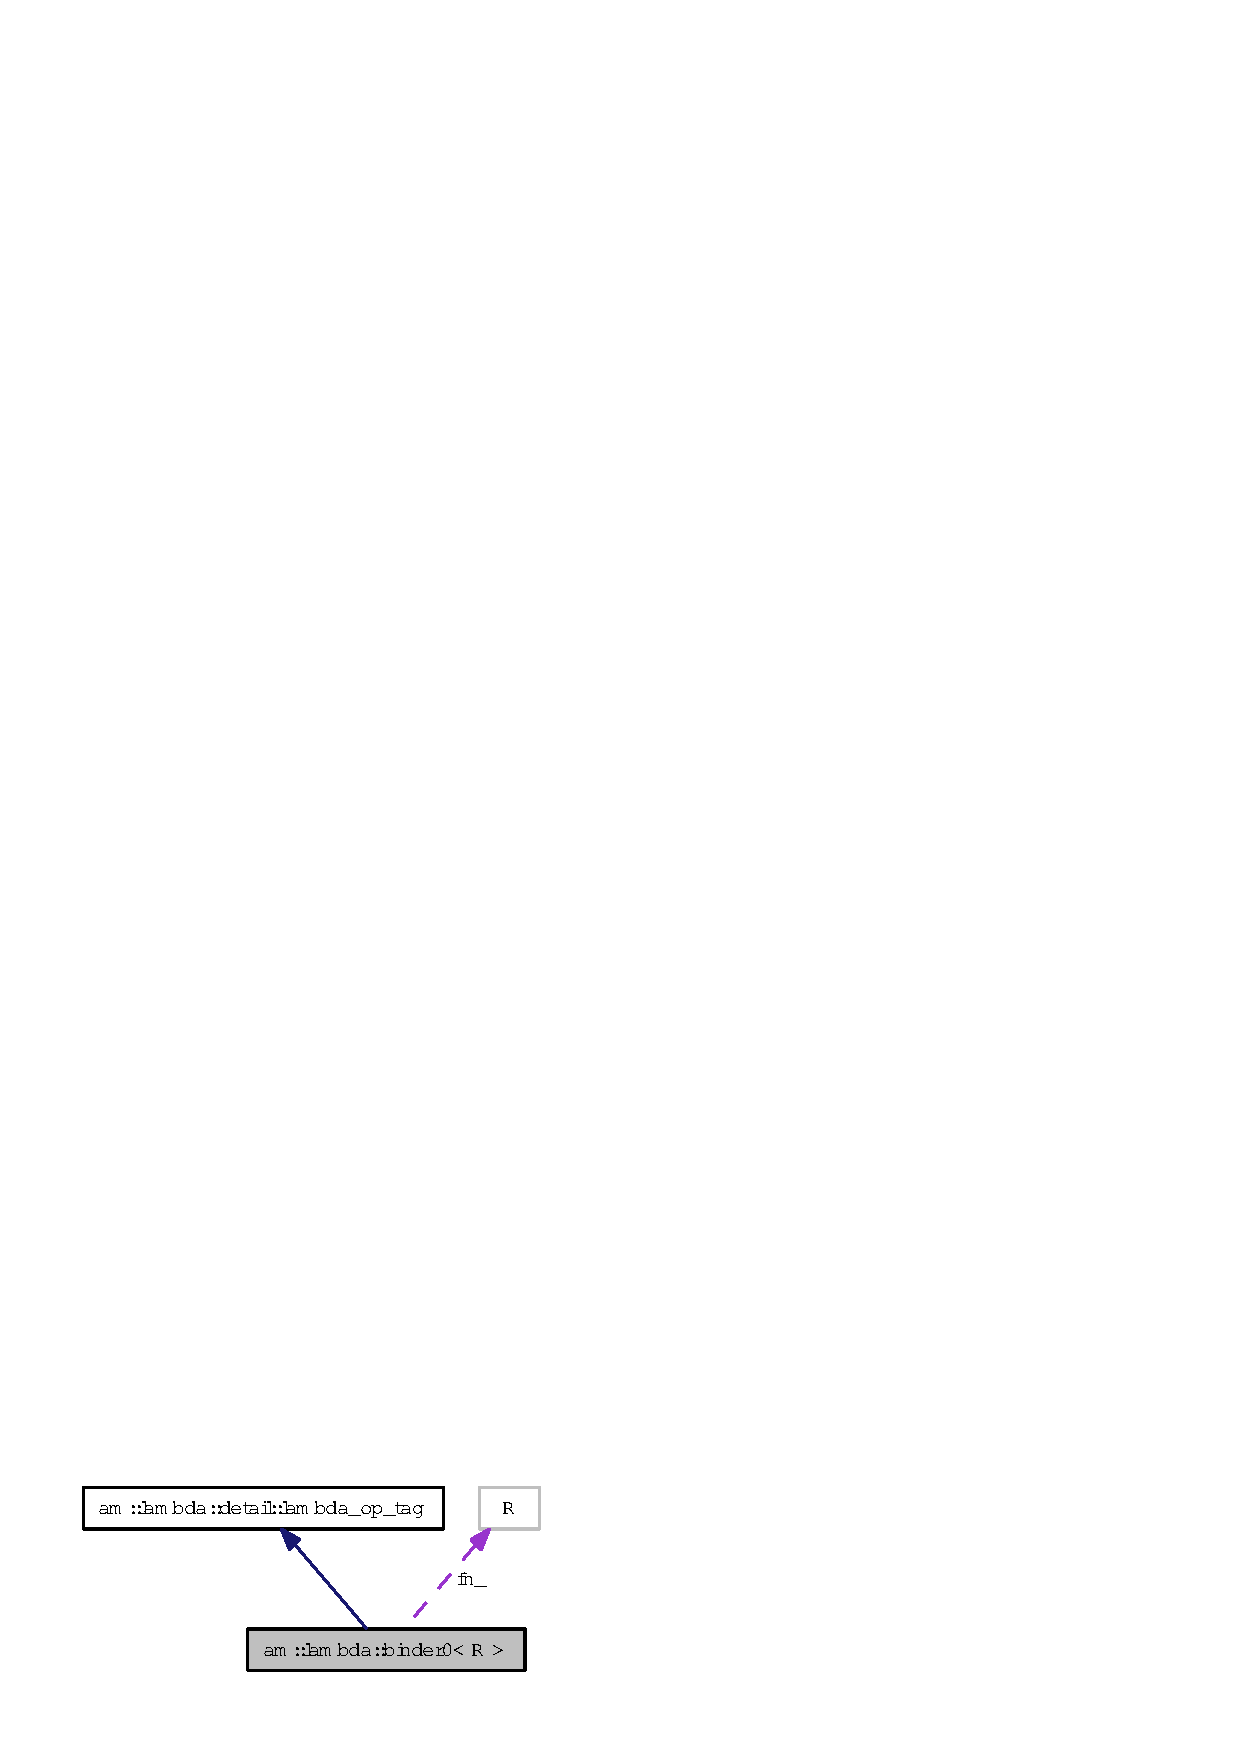
\includegraphics[width=132pt]{structam_1_1lambda_1_1binder0__coll__graph}
\end{center}
\end{figure}
\subsection*{Public Types}
\begin{CompactItemize}
\item 
typedef detail::binder\_\-impl$<$ R $>$::result\_\-type \textbf{result\_\-type}\label{structam_1_1lambda_1_1binder0_dd9b026043ecf5fa477ed0a887e0cae3}

\end{CompactItemize}
\subsection*{Public Member Functions}
\begin{CompactItemize}
\item 
\textbf{binder0} (R($\ast$fn)())\label{structam_1_1lambda_1_1binder0_503871dd93616d4b9fef28c3fcb59794}

\item 
template$<$class T1, class T2, class T3$>$ result\_\-type \textbf{operator()} (T1 t1, T2 t2, T3 t3) const \label{structam_1_1lambda_1_1binder0_140466dec5fe7965454887eea6ccc01b}

\item 
template$<$class T1, class T2$>$ result\_\-type \textbf{operator()} (T1 t1, T2 t2) const\label{structam_1_1lambda_1_1binder0_e6af6516938a98c05aa3f74b296c01d9}

\item 
template$<$class T1$>$ result\_\-type \textbf{operator()} (T1 t1) const \label{structam_1_1lambda_1_1binder0_69732777801aca26cb708730366b78bb}

\item 
result\_\-type \textbf{operator()} () const\label{structam_1_1lambda_1_1binder0_bf97e5aae6c88c14a03775ae1458d037}

\end{CompactItemize}
\subsection*{Public Attributes}
\begin{CompactItemize}
\item 
R($\ast$ \textbf{fn\_\-} )()\label{structam_1_1lambda_1_1binder0_1d5bd3720645f4288bfe02e1658cfcd0}

\end{CompactItemize}


\subsection{Detailed Description}
\subsubsection*{template$<$typename R$>$ struct am::lambda::binder0$<$ R $>$}

Binder for the free function which takes no argument. 



The documentation for this struct was generated from the following file:\begin{CompactItemize}
\item 
{\bf lambda.hpp}\end{CompactItemize}
